\documentclass[a4paper,11pt,twoside]{scrreprt}

\usepackage[utf8]{inputenc}
\usepackage[T1]{fontenc}   
\usepackage{graphicx}       
\usepackage[german]{babel}
\usepackage{csquotes}     
\usepackage{acronym}
\usepackage{eurosym}
\usepackage[linktocpage=true]{hyperref}
\usepackage[bindingoffset=8mm]{geometry}
\usepackage{caption}
\captionsetup{format=hang, justification=raggedright}
\usepackage[style=authoryear, backend=biber]{biblatex}
\usepackage{float}
\usepackage{rotating}
\usepackage{blkarray}
\usepackage{amsmath}
\usepackage{amssymb}
\usepackage{gensymb}
\usepackage{amsthm}
\newtheorem{theorem}{Theorem}[section]
\newtheorem{lemma}[theorem]{Lemma}
\usepackage{listings}
\addbibresource{references.bib} 
\usepackage{caption}
\usepackage{subcaption}

\newcommand{\argmin}[1]{\underset{#1}{\operatorname{arg}\,\operatorname{min}}\;}
\newcommand{\norm}[1]{\lVert#1\rVert}
\newcommand{\Lagr}{\mathcal{L}}

\begin{document}

% Titelblatt:
% \newpage\mbox{}\newpage
\cleardoublepage   % force output to a right page
\thispagestyle{empty}
\begin{titlepage}
  \begin{flushright}
  
\includegraphics[width=0.4\linewidth]{assets/Logo-A3.jpg}
  \end{flushright}
  \begin{center}
  \section*{Support Vector Machines (SVM)}
  \vspace{2cm}

\textbf{Computational Intelligence II}    
\vspace{0.5cm}

  Informatik - Software and Information Engineering\\
  Fachhochschule Vorarlberg\\

  \vspace{1cm}
  
    Erstellt von\\
  André Hopfgartner \& Matthias Rupp\\
  
 
  \vspace{1cm}
  

  
  Dornbirn, am \today
  
  
  \end{center}
\end{titlepage}


% Inhaltsverzeichnis:
\clearpage   % force output to a right page
\setcounter{tocdepth}{2}
\setcounter{secnumdepth}{4}
\tableofcontents

% evtl. Abkürzungsverzeichnis:
\clearpage
\phantomsection
\addcontentsline{toc}{chapter}{Abkürzungsverzeichnis}
\chapter*{Abkürzungsverzeichnis}
\begin{acronym}
 \acro{SVM}{Support Vector Machine}
\end{acronym}



\chapter{Einführung}

\section{Intuition}
Ziel: möglichst breites Band zwischen den 2 verschiedenen Klassen aufziehen.

\section{Mathematische Herleitung}

TODO TEXT HERE
\subsection{Problemdefinition}
Gegeben sei ein Gewichtsvektor $w \in \mathbb{R}^{D}$, ein Bias $b \in \mathbb{R}$, ein beliebiger Punkt $x_{n} \in \mathbb{R}^{D}$ und ein zugehöriges Label $y_{n} \in \{\-1, +1\}$. Eine Ebene im Raum kann allgemein definiert werden durch:

\begin{equation} \label{plane_eq}
    \begin{aligned}
    w^{T} x_{n} + b &= 0 \\
    \end{aligned}
\end{equation}

Weiters soll für eine richtige Klassifikation gelten:
\begin{subequations} \label{decision_rules}
	\begin{alignat}{2}
		w^{T} x_{n} + b \geq +1 & \qquad & \text{ für } y_{k} = +1\\
		w^{T} x_{n} + b \leq -1 & & \text{ für } y_{k} = -1
	\end{alignat}
\end{subequations}

\autoref{decision_rules} kann weiter verallgemeinert werden durch beidseitige Multiplikation mit $y_{k}$:

\begin{subequations} \label{decision_rules2}
	\begin{alignat}{2}
		y_{k} (w^{T} x_{n} + b) \geq 1 & \qquad & \text{ für } y_{k} = +1\\
		y_{k} (w^{T} x_{n} + b) \geq 1 & & \text{ für } y_{k} = -1
	\end{alignat}
\end{subequations}

Für den Grenzfall, dass $x_{n} = \hat{x}$ genau an der Grenze der Trennebene liegt, gilt somit:
\begin{equation} \label{dec_rule}
	\begin{aligned}
		y_{k} (w^{T} \hat{x} + b) &= 1
	\end{aligned}
\end{equation}


Als nächsten Schritt bestimmen wir den euklidischen Normalabstand $D$ eines beliebigen Punkts $x_{n} \in \mathbb{R}^{D}$ zu der Ebene. Hierfür ist zuerst zu bemerken, dass $w$ normal zur definierten Ebene steht.

\begin{lemma}
	Eine Ebene sei definiert durch $w^{T} x + b = 0$. Der Vektor $w$ steht normal zu der definierten Ebene.
\end{lemma}

\begin{proof}
	Man wähle zwei Punkte $x_{1}, x_{2} \in \mathbb{R}^{D}$ die auf der Ebene liegen. Somit muss gelten:
	\begin{equation}
		\begin{aligned}
			w^{T} x_{1} + b &= 0 \\
			w^{T} x_{2} + b &= 0 \\
			w^{T} (x_{1} - x_{2}) &= 0 \leftrightarrow \norm{w^{T}} \norm{x_{1} - x_{2}} \cos(\alpha) = 0 \leftrightarrow \alpha = 90^{\circ}
		\end{aligned}
	\end{equation}
\end{proof}

Um den Normalabstand $D$ eines beliebigen Punkts $x_{n}$ zu ermitteln wählt man einen Punkt $x$, der auf der Ebene liegt, und projiziert den Vektor $(x_{n} - x)$ auf den Einheitsvektor von $w$. Weil nur der tatsächliche Abstand zur Ebene relevant ist und nicht die Richtung nimmt man den Betrag.

\begin{equation} \label{distance_to_plane}
	\begin{aligned}
		D &= | \frac{w^{T}}{\lVert w \rVert} (x_{n} - x) | = \\
		&= \frac{1}{\norm{w}} | (w^{T} x_{n} - w^{T} x) | =\\
		&= \frac{1}{\norm{w}} | (w^{T} x_{n} + b - (w^{T} x + b)) |
	\end{aligned}
\end{equation}

\begin{figure}[H]
	\centering
	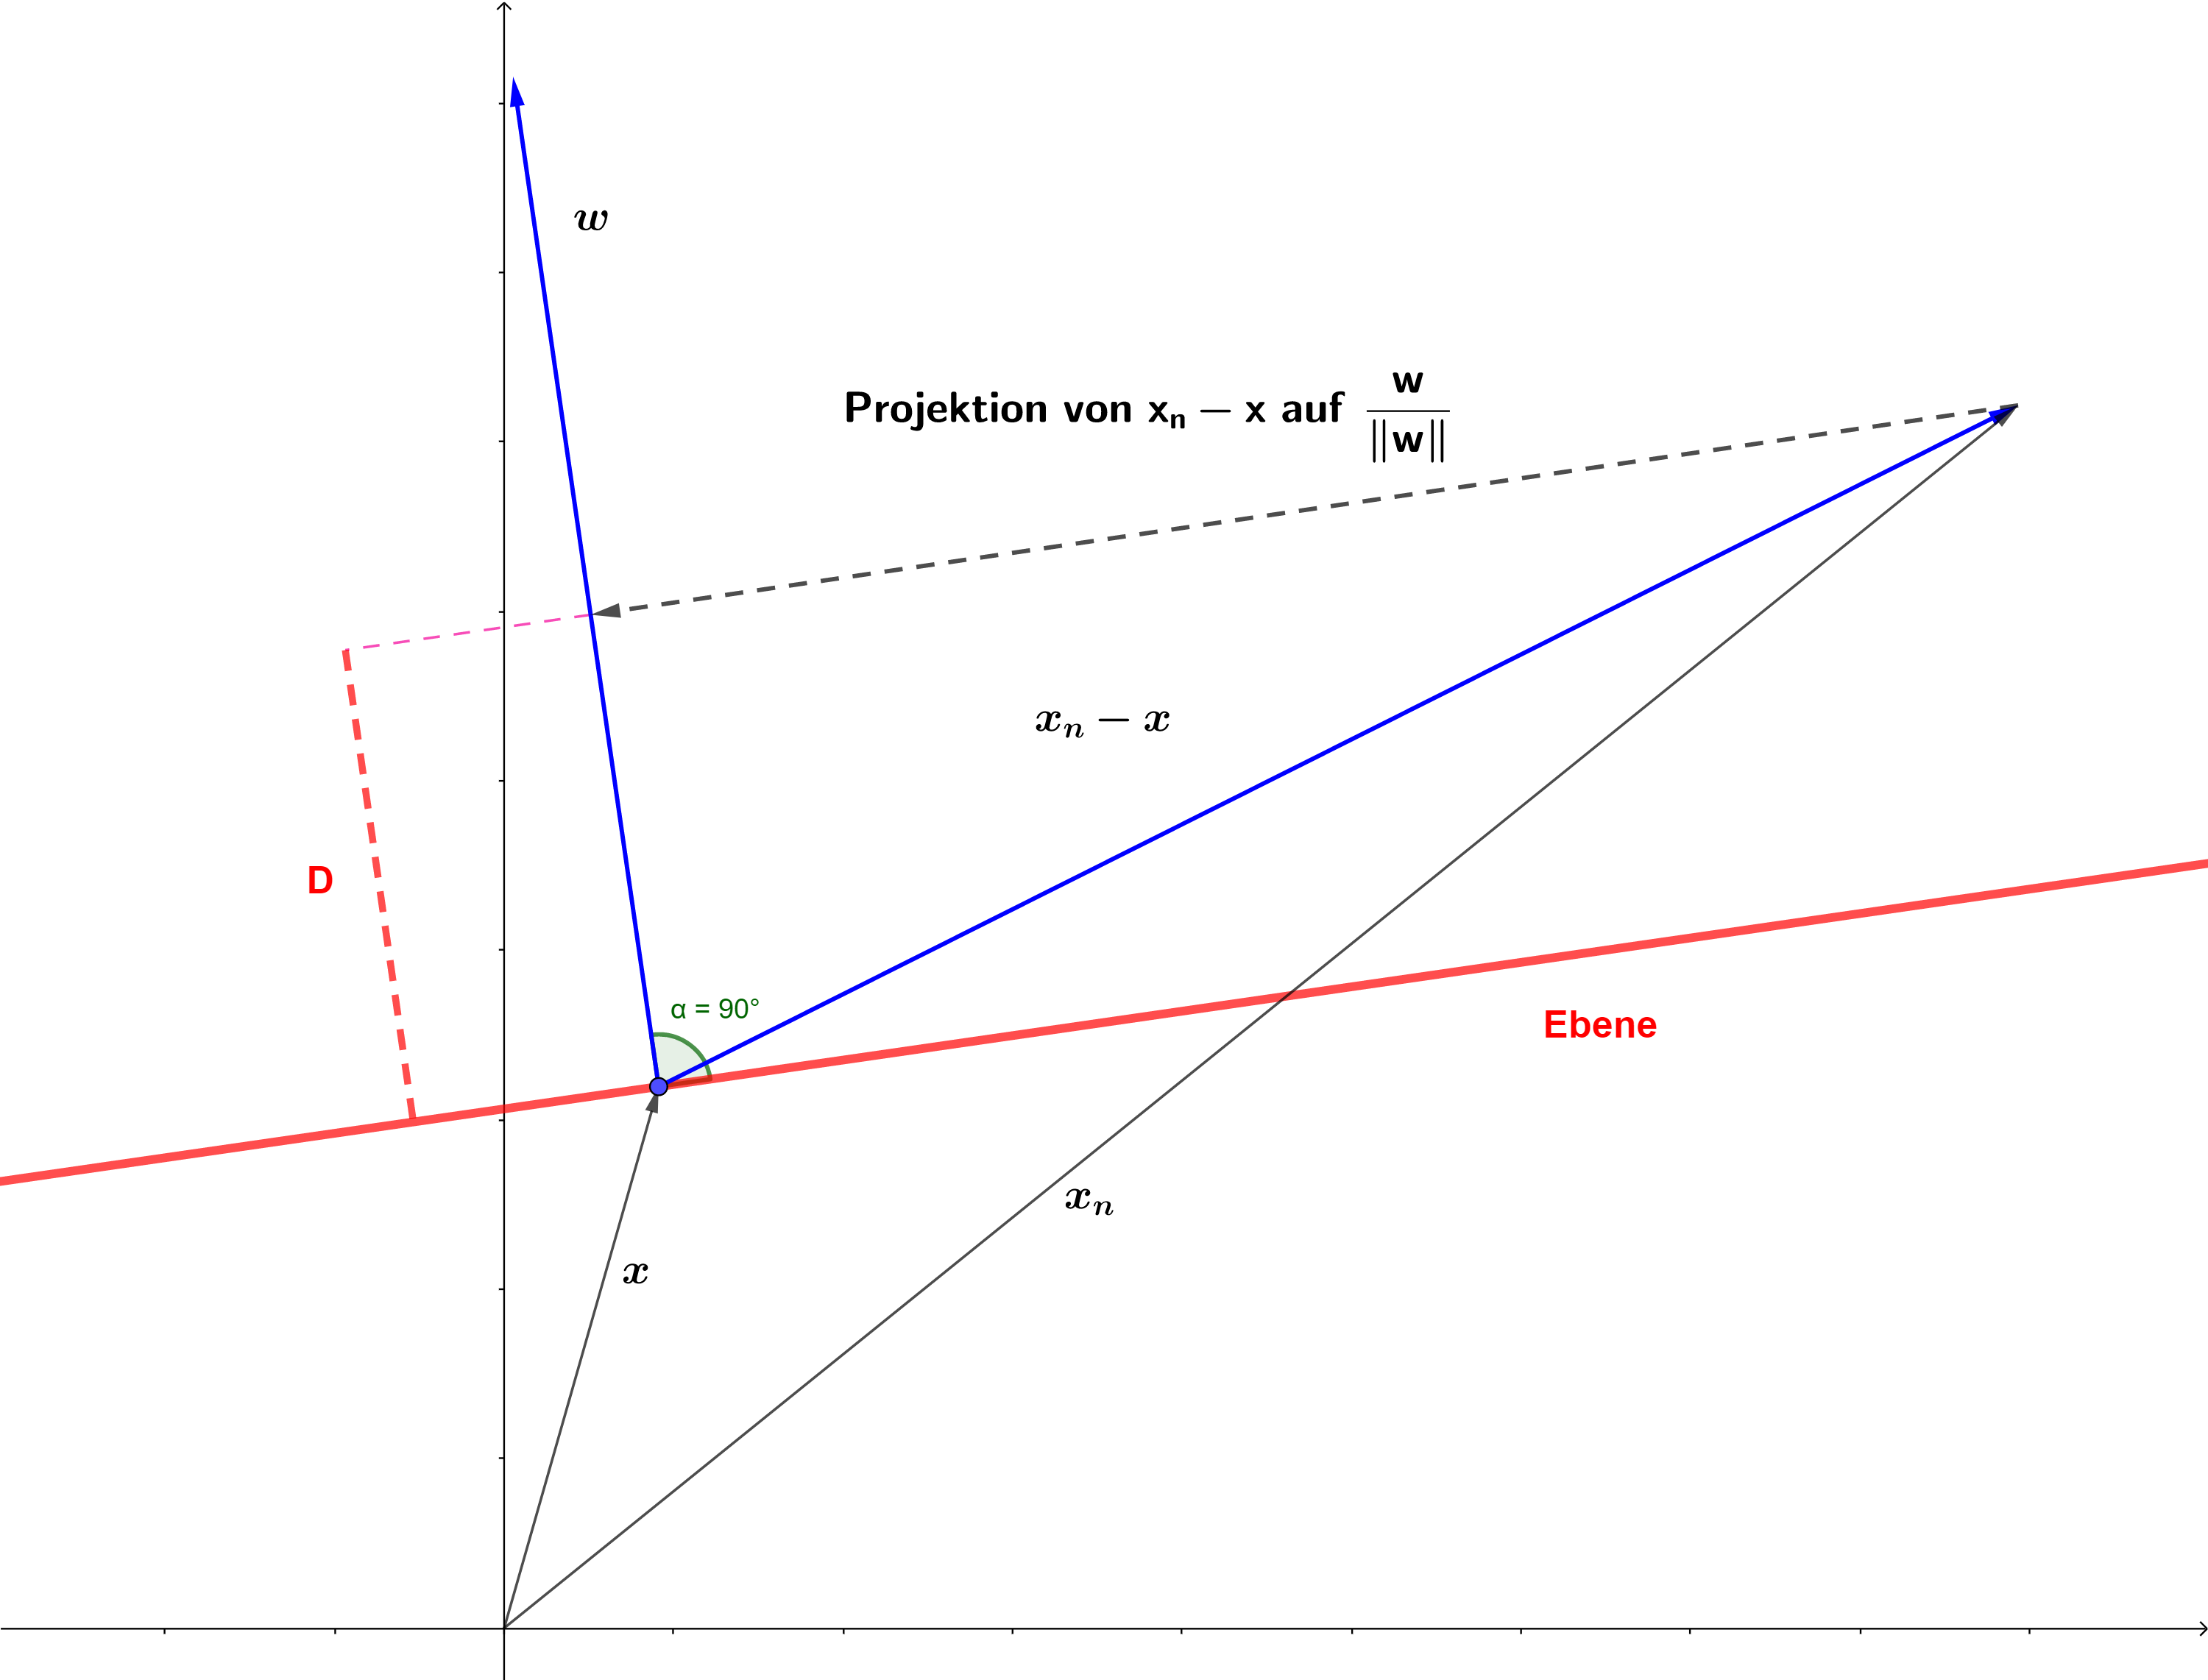
\includegraphics[width = 13cm]{assets/projection.png}
	\caption{Durch die Projektion von $(x_{n} - x)$ auf den Einheitsvektor von $w$ kann der Normalabstand $D$ von $x_{n}$ zu der Ebene bestimmt werden.}
	\label{fig:projection}
\end{figure}

Weil der Punkt $x$ auf der Ebene liegt gilt $w^{T} x + b = 0$ (\autoref{plane_eq}):
\begin{equation} \label{distance_to_plane_simplified1}
	\begin{aligned}
		D &= \frac{1}{\norm{w}} | (w^{T} x_{n} + b) |
	\end{aligned}
\end{equation}

Nun trifft man die Annahme, dass $x_{n} = \hat{x}$ der am nächsten zu der Trenngrenze liegende Punkt ist. Aus \autoref{dec_rule} gilt $y_{k} (w^{T} \hat{x} + b) = 1 = |w^{T} \hat{x} + b|$ unter der Annahme, dass der Punkt richtig klassifiziert wurde. Somit ergibt sich der kleinste Abstand zur Trennebene als:
\begin{equation} \label{distance_to_plane_simplified2}
	\begin{aligned}
		D &= \frac{1}{\norm{w}}
	\end{aligned}
\end{equation}

\subsection{Optimierungsproblem}

\autoref{distance_to_plane_simplified2} beschreibt den Normalabstand zu dem am nächsten an der Ebene liegenden Punkt $\hat{x}$. Ziel einer \ac{SVM} ist die Maximierung dieses Abstands für $N$ Eingabevektoren $\{x_{1}..x_{N}\}, x_{n} \in \mathbb{R}^{D}$. Hierbei handelt es sich um ein Optimierungsproblem mit Nebenbedingungen:

\begin{subequations}
	\begin{alignat}{2}
		&\!\max_{w}        &\qquad&  \frac{1}{\norm{w}} \label{eq:optProb}\\
		&\text{mit } &      & \min_{n=1..N} |w^{T} x_{n} + b| = 1 \label{eq:constraint1}
	\end{alignat}
\end{subequations}

\autoref{eq:constraint1} beschreibt hier den am nächsten zur Ebene gelegenen Punkt $\hat{x}$ aus der gebenenen Menge von Eingabevektoren in allgemeiner Form. Der Betrag lässt sich vermeiden durch die Anwendung von \autoref{decision_rules2}:

\begin{equation} \label{abs_value_trick}
	\begin{aligned}
		|w^{T} x_{n} + b| &= y_{n} (w^{T} x_{n} + b)
	\end{aligned}
\end{equation}


Durch Anwendung von \autoref{abs_value_trick} in \autoref{eq:constraint1}, Umformulierung der Maximierung in eine Minimierung und der Verallgemeinerung von $\hat{x}$ auf beliebige Punkte $x_{n}$ erhält man:
\begin{subequations}
	\begin{alignat}{2}
		&\!\min_{w}        &\qquad&  \frac{1}{2} w^{T} w \label{eq:optProb2}\\
		&\text{mit } &      & y_n (w^{T} x_{n} + b) \geq 1 \text{ für } n=1..N \label{eq:constraint12}
	\end{alignat}
\end{subequations}

Die Verallgemeinerung von \autoref{eq:constraint1} auf \autoref{eq:constraint12} auf beliebige Punkte ist so möglich, weil durch \autoref{dec_rule} sichergestellt ist, dass für beliebige Punkte $y_{n}(w^{T} x_{n} + b) \geq 1$ gilt.

\subsection{Lagrange Optimierung}

Das beschriebene Optimierungsproblem beinhaltet eine Ungleichung in \autoref{eq:constraint12}. Um die Lagrangegleichung aufstellen zu können wird zuerst die Nebenbedingung umgeformt:
\begin{subequations}
	\begin{alignat}{2}
		&\!\min_{w}        &\qquad&  \frac{1}{2} w^{T} w \label{eq:optProb3}\\
		&\text{mit } &      & y_n (w^{T} x_{n} + b)-1 \geq 0 \text{ für } n=1..N \label{eq:constraint13}
	\end{alignat}
\end{subequations}

Das Problem kann nun als Lagrangegleichung dargestellt werden:
\begin{subequations}
	\begin{alignat}{2}
		&\!\min_{w, b}        &\qquad&  \Lagr (w, b, \alpha) = \frac{1}{2} w^{T} w - \sum_{n=1}^{N} \alpha_{n} (y_n (w^{T} x_{n} + b)-1) \label{eq:optProb4}\\
		&\max_{\alpha_{n}} &      & \alpha_{n} \geq 0 \text{ für } n=1..N \label{eq:constraint14}
	\end{alignat}
\end{subequations}
 Weil \autoref{eq:constraint13} eine Ungleichung der Form $\geq 0$ beinhaltet werden diese Terme von der zu maximierenden Funktion subtrahiert. Nun kann die uneingeschränkte Optimierung von \autoref{eq:optProb4} nach $w$ und $b$ durchgeführt werden indem die Ableitungen bestimmt und $0$ gesetzt werden:

\begin{equation} \label{gradient_lagrange_w}
	\begin{aligned}
		\nabla_{w} \Lagr &= w - \sum_{n=1}^{N} \alpha_{n} y_{n} x_{n} \overset{!}{=} \vec{0} \\
		w &= \sum_{n=1}^{N} \alpha_{n} y_{n} x_{n}
	\end{aligned}
\end{equation}

\begin{equation} \label{partial_lagrange_b}
	\begin{aligned}
		\frac{\partial}{\partial b} \Lagr &= - \sum_{n=1}^{N} \alpha_{n} y_{n} \overset{!}{=} 0 \\
		\sum_{n=1}^{N} \alpha_{n} y_{n} &= 0
	\end{aligned}
\end{equation}

Die Ergebnisse von \autoref{gradient_lagrange_w} und \autoref{partial_lagrange_b} können in \autoref{eq:optProb4} eingesetzt werden. Hierfür wird zuerst die Summe in \autoref{eq:optProb4} in Teilsummen aufgeteilt:

\begin{equation} \label{lagrange_substituted}
	\begin{aligned}
		\Lagr(w, b, \alpha) &= \frac{1}{2} w^{T} w - \sum_{n=1}^{N} \alpha_{n} (y_n (w^{T} x_{n} + b)-1) = \\
		&= \frac{1}{2} w^{T} w - [\sum_{n=1}^{N} \alpha_{n} y_{n} b - \sum_{n=1}^{N} \alpha_{n} + \sum_{n=1}^{N} \alpha_{n} y_{n} w^{T} x_{n}]
	\end{aligned}
\end{equation}

Weil $\sum_{n=1}^{N} \alpha_{n} y_{n} = 0$ (\autoref{partial_lagrange_b}) fällt der Term $\sum_{n=1}^{N} \alpha_{n} y_{n} b$ weg:
\begin{equation} \label{lagrange_substituted2}
	\begin{aligned}
		\Lagr(w, b, \alpha) &= \frac{1}{2} w^{T} w - [-\sum_{n=1}^{N} \alpha_{n} + \sum_{n=1}^{N} \alpha_{n} y_{n} w^{T} x_{n}]
	\end{aligned}
\end{equation}

Vergleicht man den Term $\sum_{n=1}^{N} \alpha_{n} y_{n} w^{T} x_{n}$ mit dem Ergebnis von \autoref{gradient_lagrange_w} erkennt man, dass $\sum_{n=1}^{N} \alpha_{n} y_{n} w^{T} x_{n} = w^T w$ gilt. Dies kann ausgeschrieben werden als:
\begin{equation} \label{lagrange_substituted3}
	\begin{aligned}
		\Lagr(\alpha) &= \sum_{n=1}^{N }\alpha_{n} - \frac{1}{2} \sum_{n=1}^{N} \sum_{m=1}^{M} y_{n} y_{m} \alpha_{n} \alpha_{m} x_{n}^{T} x_{m}
	\end{aligned}
\end{equation}

\autoref{lagrange_substituted3} beschreibt das Optimierungsproblem ohne Abhängigkeit von $w$ und $b$, wir haben jetzt also eine Maximierung für $\alpha$ mit Nebenbedingungen:
\begin{subequations} \label{final_lagrange}
	\begin{alignat}{2}
		&\!\max_{\alpha}        &\qquad&  	\Lagr(\alpha) = \sum_{n=1}^{N} \alpha_{n} - \frac{1}{2} \sum_{n=1}^{N} \sum_{m=1}^{M} y_{n} y_{m} \alpha_{n} \alpha_{m} x_{n}^{T} x_{m} \label{eq:optProb5}\\
		&\text{mit } &      & \alpha_{n} \geq 0 \text{ für } n=1..N \label{eq:constraint16}\\
		&       & & \sum_{n=1}^{N} \alpha_{n} y_{n} = 0\text{ für } n=1..N \label{eq:constraint17}
	\end{alignat}
\end{subequations}

Das in \autoref{final_lagrange} beschriebene Problem kann beispielsweise mittels eines Quadratic Programming Solvers gelöst werden. Als Ergebnis erhält man einen Vektor $\alpha$ mit allen $\alpha_{n}$. Durch Einsetzen in $w = \sum_{n=1}^{N} \alpha_{n} y_{n} x_{n}$ kann $w$ bestimmt werden. \\

Betrachtet man den Ergebnisvektor $\alpha$ wird man feststellen, dass sehr viele Werte $0$ ergeben. In \autoref{eq:optProb4} befindet sich der Term $\alpha_{n} (y_n (w^{T} x_{n} + b)-1)$. Der Term $(y_n (w^{T} x_{n} + b)-1)$ kann als Schlupf bezeichnet werden. Das Produkt von Schlupf und $\alpha_{n}$ kann nur $0$ werden wenn entweder der Schlupf $0$ ist oder $\alpha_{n}$. Umgekehrt bedeutet dies, dass alle Vektoren, die einen minimalen Abstand zu der Trennebene haben, ein $\alpha_{n} \neq 0$ aufweisen. Vektoren, die diese Bedingung erfüllen, werden Stützvektoren genannt. \\


Mit dieser Erkenntnis kann \autoref{gradient_lagrange_w} erneut analysiert werden:

\begin{equation} \label{weights_calc}
	\begin{aligned}
		w &= \sum_{n=1}^{N} \alpha_{n} y_{n} x_{n}
	\end{aligned}
\end{equation}

Weil nur Stützvektoren ein $\alpha_{n} \neq 0$ aufweisen und somit auch nur Stützvektoren einen Beitrag zu $w$ leisten, kann \autoref{weights_calc} stark vereinfacht werden:

\begin{equation} \label{weights_calc2}
	\begin{aligned}
		w &= \sum_{n \text{ ist Stützvektor}} \alpha_{n} y_{n} x_{n}
	\end{aligned}
\end{equation}

Der Gewichtsvektor $w$ hängt also lediglich von den Stützvektoren ab, deren Anzahl in der Regel gering ist.\\


Noch offen ist die Bestimmung des Bias $b$. Weil für Stützvektoren $y_n (w^{T} x_{n} + b) = 1$ gilt (\autoref{dec_rule}) kann der Bias $b$ aus jedem beliebigen Stützvektor bestimmt werden:

\begin{equation} \label{bias_calc}
	\begin{aligned}
		b &= \frac{1}{y_{n}} - w^{T} x_{n}
	\end{aligned}
\end{equation}

\subsection{Quadratic Programming Solver}
TODO


% Literaturverzeichnis:
\clearpage
\phantomsection
\addcontentsline{toc}{chapter}{Bibliography}
\printbibliography

\end{document}
